\documentclass[]{rptuseminar}

% Specify that the source file has UTF8 encoding
\usepackage[utf8]{inputenc}
% Set up the document font; font encoding (here T1) has to fit the used font.
\usepackage[T1]{fontenc}
\usepackage{lmodern}

% Load language spec
\usepackage[american]{babel}
% German article --> ngerman (n for »neue deutsche Rechtschreibung«)
% British English --> english

% Ffor bibliography and \cite
\usepackage{cite}

% AMS extensions for math typesetting
\usepackage[intlimits]{mathtools}
\usepackage{amssymb}
% ... there are many more ...


% Load \todo command for notes
\usepackage{todonotes}
% Sebastian's favorite command for large inline todonotes
% Caveat: does not work well with \listoftodos
\newcommand\todoin[2][]{\todo[inline, caption={2do}, #1]{
		\begin{minipage}{\linewidth-1em}\noindent\relax#2\end{minipage}}}

% Load \includegraphics command for including pictures (pdf or png highly recommended)
\usepackage{graphicx}

% Typeset source/pseudo code
\usepackage{listings}

% Load TikZ library for creating graphics
% Using the PGF/TikZ manual and/or tex.stackexchange.com is highly adviced.
\usepackage{tikz}
% Load tikz libraries needed below (see the manual for a full list)
\usetikzlibrary{automata,positioning}

% Load \url command for easier hyperlinks without special link text
\usepackage{url}

% Load support for links in pdfs
\usepackage{hyperref}

% Defines default styling for code listings
\definecolor{gray_ulisses}{gray}{0.55}
\definecolor{green_ulises}{rgb}{0.2,0.75,0}
\lstset{%
  columns=flexible,
  keepspaces=true,
  tabsize=3,
  basicstyle={\fontfamily{tx}\ttfamily\small},
  stringstyle=\color{green_ulises},
  commentstyle=\color{gray_ulisses},
  identifierstyle=\slshape{},
  keywordstyle=\bfseries,
  numberstyle=\small\color{gray_ulisses},
  numberblanklines=false,
  inputencoding={utf8},
  belowskip=-1mm,
  escapeinside={//*}{\^^M} % Allow to set labels and the like in comments
}

% Defines a custom environment for indented shell commands
\newenvironment{displayshellcommand}{%
	\begin{quote}%
	\ttfamily%
}{%
	\end{quote}%
}

%%%%%%%%%%%%%%%%%%%%%%%%%%%%%%%%%%%%%%%%%%%%%%%%%%%%%%%%%%%%%%%%%%%%%%%%%%%%%%%

\title{Liquid Haskell}
\event{Seminar: Programming Languages in Winter term 2024/2025}
\author{Mehran Shahidi, Saba Safarnezhad
  \institute{Rheinland-Pfälzische Technische Universität Kaiserslautern-Landau, Department of Computer Science}}

%%%%%%%%%%%%%%%%%%%%%%%%%%%%%%%%%%%%%%%%%%%%%%%%%%%%%%%%%%%%%%%%%%%%%%%%%%%%%%%
\begin{document}
%%%%%%%%%%%%%%%%%%%%%%%%%%%%%%%%%%%%%%%%%%%%%%%%%%%%%%%%%%%%%%%%%%%%%%%%%%%%%%%

\maketitle

%%%%%%%%%%%%%%%%%%%%%%%%%%%%%%%%%%%%%%%%%%%%%%%%%%%%%%%%%%%%%%%%%%%%%%%%%%%%%%%

\begin{abstract}
  This report gives a brief overview of \textsc{LiquidHaskell}, a tool that extends Haskell with refinement types. 
  Refinement types are types that extends expressiveness of Haskell types systems by providing predicates that can verify
  invarients of the program. This report explains briefly how SMT solvers leveraged by \textsc{LiquidHaskell} and 
  how to use \textsc{LiquidHaskell} by providing some examples. Finally, we discuss the limitations of \textsc{LiquidHaskell} and compare it with other tools.
\end{abstract}

%%%%%%%%%%%%%%%%%%%%%%%%%%%%%%%%%%%%%%%%%%%%%%%%%%%%%%%%%%%%%%%%%%%%%%%%%%%%%%

\section{Introduction}
\label{sec:introduction}
Programming verfication is an important step in software developments. It is the process of
verifying that a program behaves as it expected. There has been a lot of research in this 
area and many tools have been developed. 
Type safety is one of the important features of programming languages that helps to prevent runtime errors.
Despite catching many errors at compile time, type systems are not powerful enough to catch all the errors.
On the other , testing is another way to verify the program, but it is not always possible to test all the possible inputs.
Consider the following example:

\begin{figure}[h]
\begin{lstlisting}[language=Haskell]
  average    :: [Int] -> Int
  average xs = sum xs `div` length xs
\end{lstlisting}
\end{figure}

One of the tools that is used in Haskell programming language is \textsc{LiquidHaskell}. \textsc{LiquidHaskell} 
(LH) extends Haskell with refinement types which are types that extend the expressiveness of Haskell.
With refinement types, we can provide invariant that the program should satisfy. 

In this report, after a short backgrouund on program verfication using SMT in section \ref{sec:background}, we will explain 
how LH works and how it uses SMT solvers to 
verify the program in section \ref{sec:lh}. Then in section \ref{sec:example} we will provide some examples how to use 
LH to verify \todo{problem name}\textbf{problem name} problem. Finally in section \ref{sec:conclusions} we 
discuss the limiations of LH and compare it with other tools.

% E.~g.~ 
% ``quoting'' is done by using two backticks and two single quotes

\section{Background}
\label{sec:background}
\begin{description}
  \item[Refinement Types] Refinement types are types that extend the expressiveness of Haskell types by providing predicates that can verify invariants of the program. 
  \item[Predicate] Predicates are haskell expressions that evaluate to boolean.
  \item[SMT Solvers] SMT solvers are used to check the satisfiability of the predicates. 
  
\end{description}
\(\{x \mid \varphi(x)\}\)
\subsection{SMT Solvers}
SMT (Satisfiability Modulo Theories) solvers are tools that can check the satisfiability of logical formulas in a specific theory.
SMT solvers extends the concept of SAT solvers by adding theories (e.g., the theory of equality, 
of integer numbers, of real numbers, of arrays, of lists, and so on) to the boolean logic \cite{clarke_satisfiability_2018}.
While SAT solvers can only check the satisfiability of boolean formulas, SMT solvers can check the satisfiability of formulas 
that contain variables from different theories. 
As an example, consider the following formula:

\begin{equation}
  \varphi = (x \lor y) \land (\lnot x \lor z)
\end{equation}

SAT solver can check the satisfiability of the formula \(\varphi\) by checking if there is an assignment for the variables \(x, y, z\).
For instance, \(x = true, y = false, z = true\) is an assignment that makes \(\varphi\) \(true\). 

On the other hand, SMT solvers can check the satisfiability of formulas that contain variables that required arithmetic theory as following formula:
Figure \ref{fig:scholar}

\begin{equation}
  x + y \leq 10 \quad and \quad x = y - 7
\end{equation}

\subsection{Z3 SMT Solvers}
\begin{figure}
			\begin{center}
				\fbox{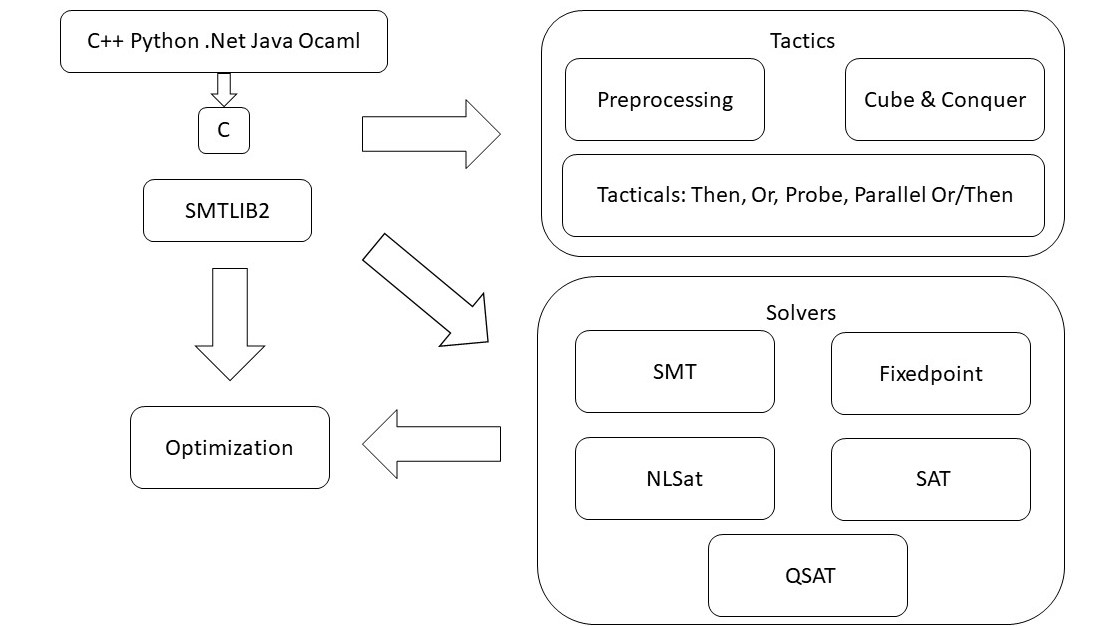
\includegraphics[width=.9\linewidth]{SMT}}%
				% fbox for "framed box"
			\end{center}
			\caption{%
         Overall system architecture of Z3
        \cite{nikolaj_bjorner_programming_nodate}
			}
			\label{fig:scholar} % NOTE: \label must appear after \caption
\end{figure}
\section{Working with LiquidHaskell}
\label{sec:lh}
\begin{lstlisting}[language=Haskell,numbers=left]
p := (e r e)                -- binary relation
   | (v e1 e2 ... en)       -- predicate (or alias) application
   | (p && p)               -- and
   | (p || p)               -- or
   | (p => p) | (p ==> p)   -- implies
   | (p <=> p)              -- iff
   | (not p)                -- negation
   | true | True
   | false | False
\end{lstlisting}
\begin{figure}
\caption{A simple example of LiquidHaskell. in line \ref{srcline:typerefinement} we define the type refinement.}
\label{alg:example}
\end{figure}
\begin{lstlisting}[language=Haskell,numbers=left]
{-# OPTIONS_GHC -fplugin=LiquidHaskell #-}

{-@ type Pos = {v:Int | 0 < v} @-}

{-@ incr :: Pos -> Pos @-} //*\label{srcline:typerefinement}
incr :: Int -> Int
incr x = x + 1 
\end{lstlisting}
\section{Example Application}
\label{sec:example}

\section{Conclusions, Results, Discussion}
\label{sec:conclusions}

%%%%%%%%%%%%%%%%%%%%%%%%%%%%%%%%%%%%%%%%%%%%%%%%%%%%%%%%%%%%%%%%%%%%%%%%%%%%%%%
\newpage
\nocite{*}
\bibliographystyle{eptcs}
\bibliography{references}

%%%%%%%%%%%%%%%%%%%%%%%%%%%%%%%%%%%%%%%%%%%%%%%%%%%%%%%%%%%%%%%%%%%%%%%%%%%%%%%
\end{document}
%%%%%%%%%%%%%%%%%%%%%%%%%%%%%%%%%%%%%%%%%%%%%%%%%%%%%%%%%%%%%%%%%%%%%%%%%%%%%%%
